\documentclass[10pt,a4paper]{article}

% Packages essentiels
\usepackage[utf8]{inputenc}
\usepackage[T1]{fontenc}
\usepackage[margin=1.5cm]{geometry}
\usepackage{amsmath,amssymb}
\usepackage{tikz}
\usetikzlibrary{positioning,calc,arrows.meta,shapes.geometric,patterns}
\usepackage{xcolor}
\usepackage{listings}
\usepackage{tcolorbox}
\tcbuselibrary{breakable}
\usepackage{hyperref}
\usepackage{multirow}
\usepackage{array}

% Configuration listings avec gestion complète des accents
\lstset{
    language=C,
    basicstyle=\ttfamily\scriptsize,
    backgroundcolor=\color{gray!10},
    keywordstyle=\color{blue},
    commentstyle=\color{gray},
    stringstyle=\color{red},
    numbers=left,
    numberstyle=\tiny,
    breaklines=true,
    frame=single,
    tabsize=4,
    showstringspaces=false,
    inputencoding=utf8,
    extendedchars=true,
    literate={é}{{\'e}}1 {è}{{\`e}}1 {à}{{\`a}}1 {ç}{{\c{c}}}1 
             {ê}{{\^e}}1 {î}{{\^i}}1 {ô}{{\^o}}1 {û}{{\^u}}1 {ù}{{\`u}}1
             {É}{{\'E}}1 {È}{{\`E}}1 {À}{{\`A}}1 {Ç}{{\c{C}}}1
             {Ê}{{\^E}}1 {Î}{{\^I}}1 {Ô}{{\^O}}1 {Û}{{\^U}}1 {Ù}{{\`U}}1
             {ë}{{\"e}}1 {ï}{{\"\i}}1 {ö}{{\"o}}1 {ü}{{\"u}}1
             {Ë}{{\"E}}1 {Ï}{{\"I}}1 {Ö}{{\"O}}1 {Ü}{{\"U}}1
             {œ}{{\oe}}1 {Œ}{{\OE}}1 {æ}{{\ae}}1 {Æ}{{\AE}}1
}

% Boxes pédagogiques
\newtcolorbox{definitionbox}[1]{
    colback=blue!5,colframe=blue!75!black,
    fonttitle=\bfseries,title=#1,breakable
}

\newtcolorbox{examplebox}[1]{
    colback=green!5,colframe=green!50!black,
    fonttitle=\bfseries,title=#1,breakable
}

\newtcolorbox{warningbox}[1]{
    colback=red!5,colframe=red!75!black,
    fonttitle=\bfseries,title=#1,breakable
}

\newtcolorbox{techbox}[1]{
    colback=orange!5,colframe=orange!75!black,
    fonttitle=\bfseries,title=#1,breakable
}

\newtcolorbox{infobox}[1]{
    colback=cyan!5,colframe=cyan!75!black,
    fonttitle=\bfseries,title=#1,breakable
}

\title{\textbf{Chapitre 3 : Structures et Unions}\\
\large Programmation C Avancée - L3}
\author{Dr. El Hadji Bassirou TOURÉ\\
Département de Mathématiques et Informatique\\
Faculté des Sciences et Techniques\\
Université Cheikh Anta Diop de Dakar}
\date{}

\begin{document}

\maketitle

\section{Structures}

\subsection{Déclaration et Définition}

Une structure est un type composé regroupant des variables de types différents sous un même nom. La déclaration définit le layout mémoire.

\begin{lstlisting}
// Déclaration de structure
struct Point {
    int x;
    int y;
};

// Définition de variable
struct Point p1;

// Déclaration + définition simultanée
struct Point p2 = {10, 20};
\end{lstlisting}

\begin{definitionbox}{Syntaxe de déclaration}
\begin{lstlisting}
struct nom_structure {
    type1 membre1;
    type2 membre2;
    // ...
};
\end{lstlisting}
La structure crée un nouveau type. Chaque membre a un offset fixe par rapport au début de la structure.
\end{definitionbox}

\subsection{Initialisation}

\begin{lstlisting}
// Initialisation positionnelle
struct Point p1 = {10, 20};

// Initialisation désignée (C99)
struct Point p2 = {.y = 20, .x = 10};

// Initialisation partielle (membres restants à 0)
struct Point p3 = {.x = 5};  // y = 0

// Initialisation composée (compound literal, C99)
struct Point p4 = (struct Point){100, 200};
\end{lstlisting}

\begin{techbox}{Initialisation désignée (C99)}
Les designated initializers permettent d'initialiser les membres dans n'importe quel ordre et de n'initialiser qu'un sous-ensemble. Les membres non spécifiés sont initialisés à zéro.
\end{techbox}

\subsection{Accès aux Membres}

\begin{lstlisting}
struct Point p = {10, 20};
struct Point *ptr = &p;

// Accès direct (opérateur .)
int a = p.x;       // a = 10

// Accès via pointeur (opérateur ->)
int b = ptr->y;    // b = 20

// Équivalence: ptr->membre == (*ptr).membre
int c = (*ptr).x;  // c = 10
\end{lstlisting}

\begin{center}
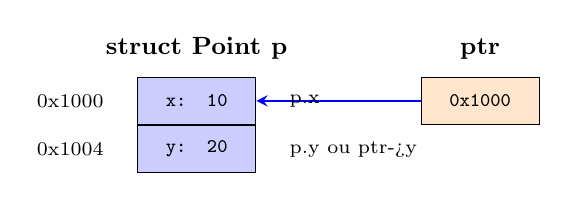
\begin{tikzpicture}[scale=0.9,
    mem/.style={rectangle,draw,minimum width=1.5cm,minimum height=0.6cm,font=\scriptsize\ttfamily},
    ptr/.style={->,>=stealth,thick}]

% Structure en mémoire
\node[mem,fill=blue!20] (x) at (0,0) {x: 10};
\node[mem,fill=blue!20,below=0pt of x] (y) {y: 20};
\node[left=0.3cm of x,font=\scriptsize] {0x1000};
\node[left=0.3cm of y,font=\scriptsize] {0x1004};
\node[above=0.1cm of x,font=\small\bfseries] {struct Point p};

% Pointeur
\node[mem,fill=orange!20] (ptr) at (4,0) {0x1000};
\node[above=0.1cm of ptr,font=\small\bfseries] {ptr};

\draw[ptr,blue] (ptr.west) -- ++(-0.5,0) |- (x.east);

% Annotations
\node[right=0.3cm of x,font=\scriptsize] {p.x};
\node[right=0.3cm of y,font=\scriptsize] {p.y ou ptr->y};

\end{tikzpicture}
\end{center}

\subsection{typedef}

\begin{lstlisting}
// Sans typedef
struct Point {
    int x, y;
};
struct Point p1;  // mot-clé struct requis

// Avec typedef
typedef struct {
    int x, y;
} Point;
Point p2;  // plus besoin de struct

// typedef avec nom de structure (pour auto-référence)
typedef struct Node {
    int data;
    struct Node *next;  // auto-référence
} Node;
\end{lstlisting}

\section{Alignement et Padding}

\subsection{Règles d'Alignement}

Les processeurs modernes imposent des contraintes d'alignement pour des raisons de performance. Un type de taille $n$ octets doit généralement être aligné sur une adresse multiple de $n$.

\begin{definitionbox}{Contraintes d'alignement (x86-64)}
\begin{center}
\begin{tabular}{|l|c|c|}
\hline
\textbf{Type} & \textbf{Taille (octets)} & \textbf{Alignement} \\
\hline
\texttt{char} & 1 & 1 \\
\texttt{short} & 2 & 2 \\
\texttt{int} & 4 & 4 \\
\texttt{long} & 8 & 8 \\
\texttt{float} & 4 & 4 \\
\texttt{double} & 8 & 8 \\
\texttt{pointeur} & 8 & 8 \\
\hline
\end{tabular}
\end{center}
L'alignement d'une structure est celui de son membre le plus contraignant.
\end{definitionbox}

\subsection{Calcul du Padding}

Le compilateur insère des octets de padding pour respecter l'alignement de chaque membre.

\begin{lstlisting}
struct S1 {
    char a;     // offset 0, size 1
    int b;      // offset 4 (padding: 3), size 4
    char c;     // offset 8, size 1
};              // taille totale: 12 (padding final: 3)
\end{lstlisting}

\begin{center}
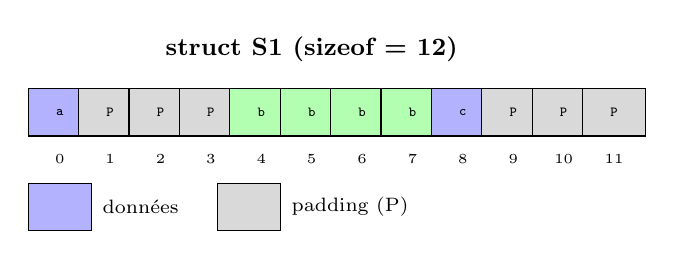
\begin{tikzpicture}[scale=0.8,
    byte/.style={rectangle,draw,minimum width=0.8cm,minimum height=0.6cm,font=\tiny\ttfamily}]

% Layout de S1
\node[font=\small\bfseries] at (4,1) {struct S1 (sizeof = 12)};

% Octets
\foreach \i in {0,...,11} {
    \node[byte] (b\i) at (\i*0.8,0) {};
    \node[below=0.1cm of b\i,font=\tiny] {\i};
}

% Contenu
\node[byte,fill=blue!30] at (0*0.8,0) {a};
\node[byte,fill=gray!30] at (1*0.8,0) {P};
\node[byte,fill=gray!30] at (2*0.8,0) {P};
\node[byte,fill=gray!30] at (3*0.8,0) {P};
\node[byte,fill=green!30] at (4*0.8,0) {b};
\node[byte,fill=green!30] at (5*0.8,0) {b};
\node[byte,fill=green!30] at (6*0.8,0) {b};
\node[byte,fill=green!30] at (7*0.8,0) {b};
\node[byte,fill=blue!30] at (8*0.8,0) {c};
\node[byte,fill=gray!30] at (9*0.8,0) {P};
\node[byte,fill=gray!30] at (10*0.8,0) {P};
\node[byte,fill=gray!30] at (11*0.8,0) {P};

% Légende
\node[byte,fill=blue!30] at (0,-1.5) {};
\node[right=0.1cm,font=\scriptsize] at (0.4,-1.5) {données};
\node[byte,fill=gray!30] at (3,-1.5) {};
\node[right=0.1cm,font=\scriptsize] at (3.4,-1.5) {padding (P)};

\end{tikzpicture}
\end{center}

\subsection{Optimisation par Réorganisation}

Réorganiser les membres par taille décroissante minimise le padding.

\begin{lstlisting}
// Structure non optimisée: 24 octets
struct Bad {
    char a;     // 1 + 7 padding
    double b;   // 8
    char c;     // 1 + 7 padding
};

// Structure optimisée: 16 octets
struct Good {
    double b;   // 8
    char a;     // 1
    char c;     // 1 + 6 padding
};
\end{lstlisting}

\begin{center}
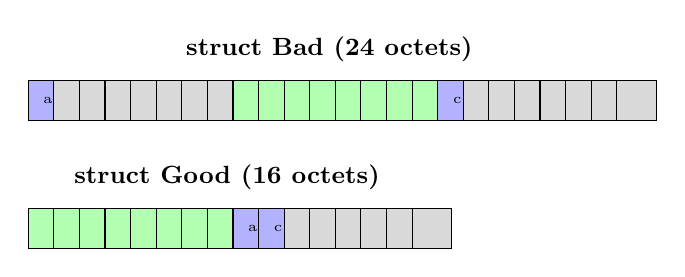
\begin{tikzpicture}[scale=0.65,
    byte/.style={rectangle,draw,minimum width=0.5cm,minimum height=0.5cm,font=\tiny}]

% Bad structure
\node[font=\small\bfseries] at (5.5,1.5) {struct Bad (24 octets)};
\foreach \i in {0,...,23} {
    \node[byte] (bad\i) at (\i*0.5,0.5) {};
}
\node[byte,fill=blue!30] at (0*0.5,0.5) {a};
\foreach \i in {1,...,7} { \node[byte,fill=gray!30] at (\i*0.5,0.5) {}; }
\foreach \i in {8,...,15} { \node[byte,fill=green!30] at (\i*0.5,0.5) {}; }
\node[byte,fill=blue!30] at (16*0.5,0.5) {c};
\foreach \i in {17,...,23} { \node[byte,fill=gray!30] at (\i*0.5,0.5) {}; }

% Good structure
\node[font=\small\bfseries] at (3.5,-1) {struct Good (16 octets)};
\foreach \i in {0,...,15} {
    \node[byte] (good\i) at (\i*0.5,-2) {};
}
\foreach \i in {0,...,7} { \node[byte,fill=green!30] at (\i*0.5,-2) {}; }
\node[byte,fill=blue!30] at (8*0.5,-2) {a};
\node[byte,fill=blue!30] at (9*0.5,-2) {c};
\foreach \i in {10,...,15} { \node[byte,fill=gray!30] at (\i*0.5,-2) {}; }

\end{tikzpicture}
\end{center}

\subsection{Représentation Hexadécimale}

\begin{examplebox}{Analyse forensique d'une structure}
\begin{lstlisting}
struct Data {
    char tag;       // offset 0
    int value;      // offset 4
    short flags;    // offset 8
};
struct Data d = {'A', 0x12345678, 0xABCD};
\end{lstlisting}

Dump mémoire (little-endian, adresse 0x1000):
\begin{verbatim}
0x1000: 41 00 00 00 78 56 34 12 CD AB 00 00
        ^  ^--padding  ^--value     ^--flags ^--padding
        tag
\end{verbatim}
\end{examplebox}

\begin{center}
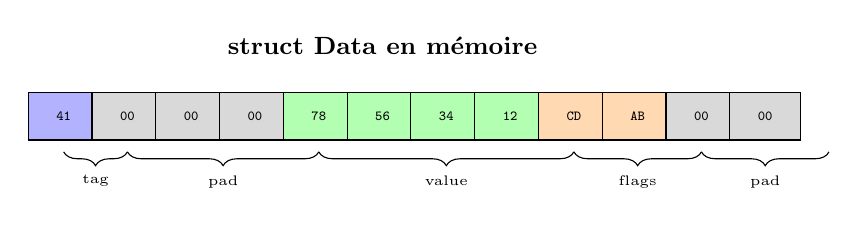
\begin{tikzpicture}[scale=0.9,
    byte/.style={rectangle,draw,minimum width=0.9cm,minimum height=0.6cm,font=\tiny\ttfamily}]

\node[font=\small\bfseries] at (4.5,1) {struct Data en mémoire};

% Adresses et valeurs hex
\foreach \i/\val in {0/41,1/00,2/00,3/00,4/78,5/56,6/34,7/12,8/CD,9/AB,10/00,11/00} {
    \node[byte] (b\i) at (\i*0.9,0) {\val};
}

% Coloration
\node[byte,fill=blue!30] at (0*0.9,0) {41};
\node[byte,fill=gray!30] at (1*0.9,0) {00};
\node[byte,fill=gray!30] at (2*0.9,0) {00};
\node[byte,fill=gray!30] at (3*0.9,0) {00};
\node[byte,fill=green!30] at (4*0.9,0) {78};
\node[byte,fill=green!30] at (5*0.9,0) {56};
\node[byte,fill=green!30] at (6*0.9,0) {34};
\node[byte,fill=green!30] at (7*0.9,0) {12};
\node[byte,fill=orange!30] at (8*0.9,0) {CD};
\node[byte,fill=orange!30] at (9*0.9,0) {AB};
\node[byte,fill=gray!30] at (10*0.9,0) {00};
\node[byte,fill=gray!30] at (11*0.9,0) {00};

% Annotations
\draw[decorate,decoration={brace,amplitude=5pt,mirror}] (0,-0.5) -- (0.9,-0.5) node[midway,below=5pt,font=\tiny] {tag};
\draw[decorate,decoration={brace,amplitude=5pt,mirror}] (0.9,-0.5) -- (3.6,-0.5) node[midway,below=5pt,font=\tiny] {pad};
\draw[decorate,decoration={brace,amplitude=5pt,mirror}] (3.6,-0.5) -- (7.2,-0.5) node[midway,below=5pt,font=\tiny] {value};
\draw[decorate,decoration={brace,amplitude=5pt,mirror}] (7.2,-0.5) -- (9,-0.5) node[midway,below=5pt,font=\tiny] {flags};
\draw[decorate,decoration={brace,amplitude=5pt,mirror}] (9,-0.5) -- (10.8,-0.5) node[midway,below=5pt,font=\tiny] {pad};

\end{tikzpicture}
\end{center}

\section{Structures Imbriquées}

\begin{lstlisting}
struct Point {
    int x, y;
};

struct Rectangle {
    struct Point top_left;
    struct Point bottom_right;
    char color;
};

struct Rectangle r = {{0, 0}, {100, 50}, 'R'};

// Accès
int x1 = r.top_left.x;
int y2 = r.bottom_right.y;
\end{lstlisting}

\begin{center}
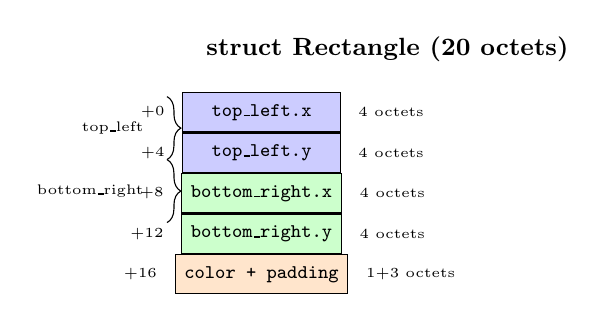
\begin{tikzpicture}[scale=0.8,
    mem/.style={rectangle,draw,minimum width=2cm,minimum height=0.5cm,font=\scriptsize\ttfamily}]

\node[font=\small\bfseries] at (2,2) {struct Rectangle (20 octets)};

\node[mem,fill=blue!20] (tl_x) at (0,1) {top\_left.x};
\node[mem,fill=blue!20,below=0pt of tl_x] (tl_y) {top\_left.y};
\node[mem,fill=green!20,below=0pt of tl_y] (br_x) {bottom\_right.x};
\node[mem,fill=green!20,below=0pt of br_x] (br_y) {bottom\_right.y};
\node[mem,fill=orange!20,below=0pt of br_y] (color) {color + padding};

% Offsets
\node[left=0.1cm of tl_x,font=\tiny] {+0};
\node[left=0.1cm of tl_y,font=\tiny] {+4};
\node[left=0.1cm of br_x,font=\tiny] {+8};
\node[left=0.1cm of br_y,font=\tiny] {+12};
\node[left=0.1cm of color,font=\tiny] {+16};

% Tailles
\node[right=0.1cm of tl_x,font=\tiny] {4 octets};
\node[right=0.1cm of tl_y,font=\tiny] {4 octets};
\node[right=0.1cm of br_x,font=\tiny] {4 octets};
\node[right=0.1cm of br_y,font=\tiny] {4 octets};
\node[right=0.1cm of color,font=\tiny] {1+3 octets};

% Accolades
\draw[decorate,decoration={brace,amplitude=5pt}] (-1.5,1.25) -- (-1.5,0.25) node[midway,left=5pt,font=\tiny] {top\_left};
\draw[decorate,decoration={brace,amplitude=5pt}] (-1.5,0.25) -- (-1.5,-0.75) node[midway,left=5pt,font=\tiny] {bottom\_right};

\end{tikzpicture}
\end{center}

\subsection{Tableaux de Structures}

\begin{lstlisting}
struct Point points[3] = {{0,0}, {10,20}, {30,40}};

// Accès
int x1 = points[1].x;     // 10
int y2 = points[2].y;     // 40

// Via pointeur
struct Point *p = points;
int x0 = p->x;            // 0
int x1 = (p+1)->x;        // 10
\end{lstlisting}

\begin{center}
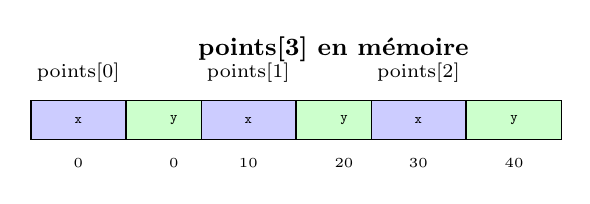
\begin{tikzpicture}[scale=0.9,
    cell/.style={rectangle,draw,minimum width=1.2cm,minimum height=0.5cm,font=\tiny\ttfamily}]

\node[font=\small\bfseries] at (3.6,1) {points[3] en mémoire};

% Points
\foreach \i in {0,1,2} {
    \node[cell,fill=blue!20] (x\i) at (\i*2.4,0) {x};
    \node[cell,fill=green!20,right=0pt of x\i] (y\i) {y};
}

% Valeurs
\node[below=0.1cm of x0,font=\tiny] {0};
\node[below=0.1cm of y0,font=\tiny] {0};
\node[below=0.1cm of x1,font=\tiny] {10};
\node[below=0.1cm of y1,font=\tiny] {20};
\node[below=0.1cm of x2,font=\tiny] {30};
\node[below=0.1cm of y2,font=\tiny] {40};

% Indices
\node[above=0.1cm of x0,font=\scriptsize] {points[0]};
\node[above=0.1cm of x1,font=\scriptsize] {points[1]};
\node[above=0.1cm of x2,font=\scriptsize] {points[2]};

\end{tikzpicture}
\end{center}

\section{Unions}

\subsection{Définition et Caractéristiques}

Une union est un type composé où tous les membres partagent la même zone mémoire. La taille de l'union est celle de son plus grand membre.

\begin{lstlisting}
union Data {
    int i;
    float f;
    char c[4];
};

union Data d;
d.i = 0x41424344;
printf("%c%c%c%c\n", d.c[0], d.c[1], d.c[2], d.c[3]);
// Affiche: DCBA (little-endian)
\end{lstlisting}

\begin{center}
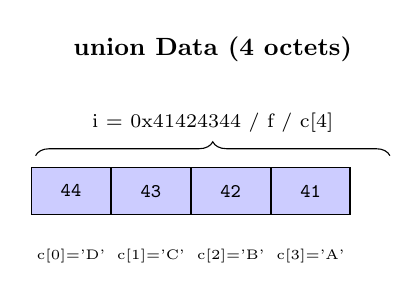
\begin{tikzpicture}[scale=0.9,
    byte/.style={rectangle,draw,minimum width=1cm,minimum height=0.6cm,font=\scriptsize\ttfamily}]

\node[font=\small\bfseries] at (2,2) {union Data (4 octets)};

% Représentation superposée
\node[byte,fill=blue!20] (b0) at (0,0) {44};
\node[byte,fill=blue!20,right=0pt of b0] (b1) {43};
\node[byte,fill=blue!20,right=0pt of b1] (b2) {42};
\node[byte,fill=blue!20,right=0pt of b2] (b3) {41};

% Annotations
\node[below=0.3cm of b0,font=\tiny] {c[0]='D'};
\node[below=0.3cm of b1,font=\tiny] {c[1]='C'};
\node[below=0.3cm of b2,font=\tiny] {c[2]='B'};
\node[below=0.3cm of b3,font=\tiny] {c[3]='A'};

\draw[decorate,decoration={brace,amplitude=5pt}] (-0.5,0.5) -- (4.5,0.5) node[midway,above=5pt,font=\scriptsize] {i = 0x41424344 / f / c[4]};

\end{tikzpicture}
\end{center}

\begin{warningbox}{Type Punning}
Accéder à un membre différent de celui qui a été écrit en dernier constitue du type punning. Le comportement est défini en C (contrairement à C++) mais peut produire des résultats dépendants de l'architecture (endianness).
\end{warningbox}

\subsection{Tagged Union (Union Discriminée)}

Pattern pour utiliser les unions de manière sûre: associer un tag indiquant le type actif.

\begin{lstlisting}
typedef enum { INT_TYPE, FLOAT_TYPE, STRING_TYPE } DataType;

typedef struct {
    DataType type;  // discriminant
    union {
        int i;
        float f;
        char *s;
    } value;
} Variant;

void print_variant(Variant *v) {
    switch (v->type) {
        case INT_TYPE:   printf("%d\n", v->value.i); break;
        case FLOAT_TYPE: printf("%f\n", v->value.f); break;
        case STRING_TYPE: printf("%s\n", v->value.s); break;
    }
}
\end{lstlisting}

\begin{center}
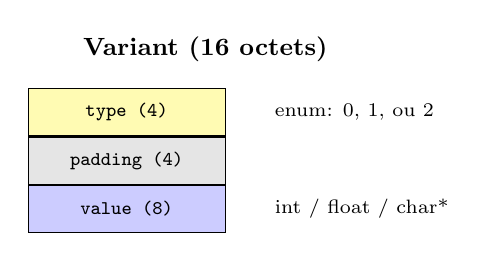
\begin{tikzpicture}[scale=0.8,
    mem/.style={rectangle,draw,minimum width=2.5cm,minimum height=0.6cm,font=\scriptsize\ttfamily}]

\node[font=\small\bfseries] at (1.25,1.5) {Variant (16 octets)};

\node[mem,fill=yellow!30] (type) at (0,0.5) {type (4)};
\node[mem,fill=gray!20,below=0pt of type] (pad) {padding (4)};
\node[mem,fill=blue!20,below=0pt of pad] (val) {value (8)};

\node[right=0.5cm of type,font=\scriptsize] {enum: 0, 1, ou 2};
\node[right=0.5cm of val,font=\scriptsize] {int / float / char*};

\end{tikzpicture}
\end{center}

\subsection{Cas d'Usage des Unions}

\begin{techbox}{Applications typiques}
\begin{itemize}
\item \textbf{Type punning}: conversion entre représentations (int $\leftrightarrow$ float)
\item \textbf{Économie mémoire}: stocker des données alternatives
\item \textbf{Protocoles réseau}: interpréter des paquets selon le type
\item \textbf{Registres hardware}: accéder à des champs de bits
\item \textbf{Variants}: implémenter des types polymorphes
\end{itemize}
\end{techbox}

\section{Champs de Bits (Bit Fields)}

Les bit fields permettent de définir des membres de structure occupant un nombre spécifique de bits.

\begin{lstlisting}
struct Flags {
    unsigned int active : 1;    // 1 bit
    unsigned int mode : 3;      // 3 bits (0-7)
    unsigned int priority : 4;  // 4 bits (0-15)
};

struct Flags f = {1, 5, 12};
// Layout possible: [priority:4][mode:3][active:1] = 0xC5
\end{lstlisting}

\begin{center}
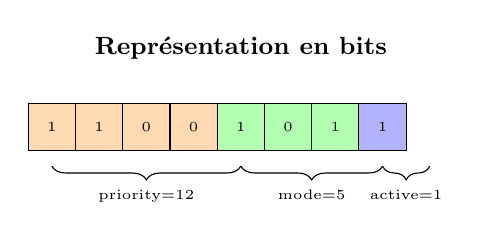
\begin{tikzpicture}[scale=1,
    bit/.style={rectangle,draw,minimum width=0.6cm,minimum height=0.6cm,font=\tiny}]

\node[font=\small\bfseries] at (2.4,1) {Représentation en bits};

% Bits (MSB à gauche)
\foreach \i/\val in {0/1,1/1,2/0,3/0,4/1,5/0,6/1,7/1} {
    \node[bit] (b\i) at (\i*0.6,0) {\val};
}

% Champs
\node[bit,fill=orange!30] at (0*0.6,0) {1};
\node[bit,fill=orange!30] at (1*0.6,0) {1};
\node[bit,fill=orange!30] at (2*0.6,0) {0};
\node[bit,fill=orange!30] at (3*0.6,0) {0};
\node[bit,fill=green!30] at (4*0.6,0) {1};
\node[bit,fill=green!30] at (5*0.6,0) {0};
\node[bit,fill=green!30] at (6*0.6,0) {1};
\node[bit,fill=blue!30] at (7*0.6,0) {1};

\draw[decorate,decoration={brace,amplitude=5pt,mirror}] (0,-0.5) -- (2.4,-0.5) node[midway,below=5pt,font=\tiny] {priority=12};
\draw[decorate,decoration={brace,amplitude=5pt,mirror}] (2.4,-0.5) -- (4.2,-0.5) node[midway,below=5pt,font=\tiny] {mode=5};
\draw[decorate,decoration={brace,amplitude=5pt,mirror}] (4.2,-0.5) -- (4.8,-0.5) node[midway,below=5pt,font=\tiny] {active=1};

\end{tikzpicture}
\end{center}

\begin{warningbox}{Portabilité des Bit Fields}
L'ordre des bits, l'alignement, et le packing des bit fields sont définis par l'implémentation. Le code utilisant des bit fields pour des protocoles réseau ou des formats de fichiers n'est pas portable. Préférer les masques et décalages explicites pour le code portable.
\end{warningbox}

\section{Structures et Allocation Dynamique}

\subsection{Allocation de Structures}

\begin{lstlisting}
#include <stdlib.h>

struct Point {
    int x, y;
};

// Allocation d'une structure
struct Point *p = malloc(sizeof(struct Point));
if (p == NULL) { /* erreur */ }
p->x = 10;
p->y = 20;
free(p);

// Allocation d'un tableau de structures
struct Point *points = malloc(5 * sizeof(struct Point));
for (int i = 0; i < 5; i++) {
    points[i].x = i;
    points[i].y = i * 2;
}
free(points);
\end{lstlisting}

\begin{center}
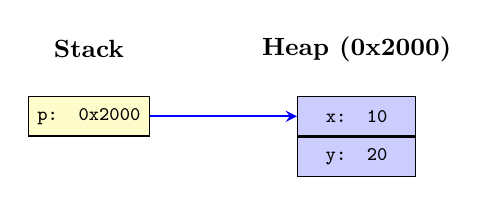
\begin{tikzpicture}[scale=0.85,
    mem/.style={rectangle,draw,minimum width=1.5cm,minimum height=0.5cm,font=\scriptsize\ttfamily},
    ptr/.style={->,>=stealth,thick}]

% Stack
\node[font=\small\bfseries] at (0,2) {Stack};
\node[mem,fill=yellow!20] (pvar) at (0,1) {p: 0x2000};

% Heap
\node[font=\small\bfseries] at (4,2) {Heap (0x2000)};
\node[mem,fill=blue!20] (px) at (4,1) {x: 10};
\node[mem,fill=blue!20,below=0pt of px] (py) {y: 20};

\draw[ptr,blue] (pvar.east) -- ++(0.5,0) |- (px.west);

\end{tikzpicture}
\end{center}

\subsection{Structures avec Membres Dynamiques}

\begin{lstlisting}
typedef struct {
    char *name;
    int *data;
    size_t size;
} Container;

Container *create_container(const char *name, size_t n) {
    Container *c = malloc(sizeof(Container));
    if (!c) return NULL;
    
    c->name = strdup(name);  // allocation pour name
    c->data = malloc(n * sizeof(int));
    c->size = n;
    
    if (!c->name || !c->data) {
        free(c->name);
        free(c->data);
        free(c);
        return NULL;
    }
    return c;
}

void destroy_container(Container *c) {
    if (c) {
        free(c->name);  // libérer les membres d'abord
        free(c->data);
        free(c);        // puis la structure
    }
}
\end{lstlisting}

\begin{center}
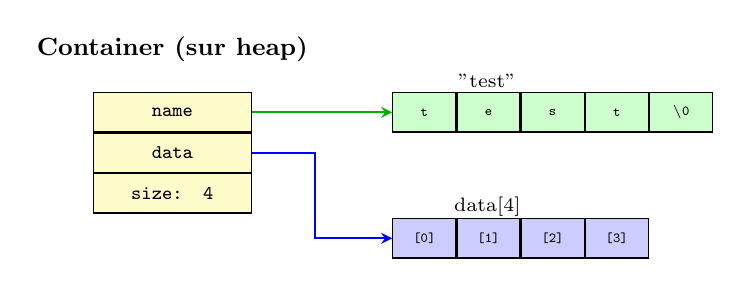
\begin{tikzpicture}[scale=0.8,
    mem/.style={rectangle,draw,minimum width=2cm,minimum height=0.5cm,font=\scriptsize\ttfamily},
    data/.style={rectangle,draw,minimum width=0.8cm,minimum height=0.5cm,font=\tiny\ttfamily},
    ptr/.style={->,>=stealth,thick}]

% Container struct
\node[font=\small\bfseries] at (0,2.5) {Container (sur heap)};
\node[mem,fill=yellow!20] (name) at (0,1.5) {name};
\node[mem,fill=yellow!20,below=0pt of name] (data) {data};
\node[mem,fill=yellow!20,below=0pt of data] (size) {size: 4};

% String
\node[font=\scriptsize] at (5,2) {"test"};
\node[data,fill=green!20] (s0) at (4,1.5) {t};
\node[data,fill=green!20,right=0pt of s0] (s1) {e};
\node[data,fill=green!20,right=0pt of s1] (s2) {s};
\node[data,fill=green!20,right=0pt of s2] (s3) {t};
\node[data,fill=green!20,right=0pt of s3] (s4) {$\backslash$0};

% Data array
\node[font=\scriptsize] at (5,0) {data[4]};
\node[data,fill=blue!20] (d0) at (4,-0.5) {[0]};
\node[data,fill=blue!20,right=0pt of d0] (d1) {[1]};
\node[data,fill=blue!20,right=0pt of d1] (d2) {[2]};
\node[data,fill=blue!20,right=0pt of d2] (d3) {[3]};

\draw[ptr,green!70!black] (name.east) -- (s0.west);
\draw[ptr,blue] (data.east) -- ++(1,0) |- (d0.west);

\end{tikzpicture}
\end{center}

\subsection{Flexible Array Member (C99)}

\begin{lstlisting}
// Membre tableau flexible (doit être le dernier)
typedef struct {
    size_t length;
    int data[];  // flexible array member
} FlexArray;

// Allocation
FlexArray *create(size_t n) {
    FlexArray *arr = malloc(sizeof(FlexArray) + n * sizeof(int));
    arr->length = n;
    return arr;
}

FlexArray *a = create(10);
a->data[0] = 42;  // accès direct
\end{lstlisting}

\begin{center}
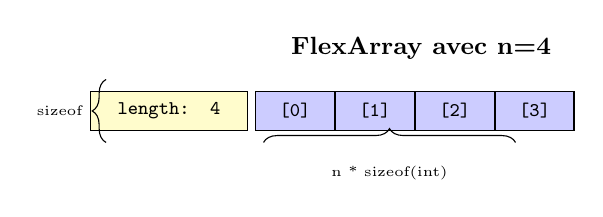
\begin{tikzpicture}[scale=0.8,
    mem/.style={rectangle,draw,minimum width=1cm,minimum height=0.5cm,font=\scriptsize\ttfamily}]

\node[font=\small\bfseries] at (4,1.5) {FlexArray avec n=4};

% Structure
\node[mem,fill=yellow!20,minimum width=2cm] (len) at (0,0.5) {length: 4};
\node[mem,fill=blue!20] (d0) at (2,0.5) {[0]};
\node[mem,fill=blue!20,right=0pt of d0] (d1) {[1]};
\node[mem,fill=blue!20,right=0pt of d1] (d2) {[2]};
\node[mem,fill=blue!20,right=0pt of d2] (d3) {[3]};

\draw[decorate,decoration={brace,amplitude=5pt}] (-1,0) -- (-1,1) node[midway,left=5pt,font=\tiny] {sizeof};
\draw[decorate,decoration={brace,amplitude=5pt}] (1.5,0) -- (5.5,0) node[midway,below=5pt,font=\tiny] {n * sizeof(int)};

\end{tikzpicture}
\end{center}

\section{Structures Opaques et Encapsulation}

\subsection{Forward Declaration}

La déclaration anticipée permet de déclarer un type sans révéler sa structure.

\begin{lstlisting}
// Dans header.h
typedef struct Stack Stack;  // forward declaration

Stack *stack_create(void);
void stack_push(Stack *s, int value);
int stack_pop(Stack *s);
void stack_destroy(Stack *s);

// Dans implementation.c
#include "header.h"

struct Stack {
    int *data;
    size_t capacity;
    size_t top;
};

Stack *stack_create(void) {
    Stack *s = malloc(sizeof(Stack));
    s->data = malloc(16 * sizeof(int));
    s->capacity = 16;
    s->top = 0;
    return s;
}
\end{lstlisting}

\begin{techbox}{Avantages de l'encapsulation}
\begin{itemize}
\item \textbf{Abstraction}: l'utilisateur manipule un pointeur opaque
\item \textbf{Évolution}: la structure interne peut changer sans modifier l'API
\item \textbf{Compilation}: modifier l'implémentation ne recompile pas les clients
\item \textbf{Sécurité}: impossible d'accéder directement aux membres
\end{itemize}
\end{techbox}

\section{Résumé des Tailles et Alignements}

\begin{center}
\begin{tabular}{|l|c|c|l|}
\hline
\textbf{Concept} & \textbf{Taille} & \textbf{Alignement} & \textbf{Notes} \\
\hline
\texttt{struct} & $\geq$ somme membres & max(membres) & + padding \\
\texttt{union} & max(membres) & max(membres) & membres superposés \\
bit field & selon déclaration & selon type & non portable \\
flexible array & 0 dans sizeof & type élément & C99 \\
\hline
\end{tabular}
\end{center}

\begin{infobox}{Outils d'inspection}
\begin{lstlisting}
// offsetof: offset d'un membre (stddef.h)
#include <stddef.h>
size_t off = offsetof(struct S, membre);

// sizeof: taille totale
size_t sz = sizeof(struct S);

// GDB: examiner une structure
(gdb) ptype struct S
(gdb) p sizeof(struct S)
(gdb) x/12xb &variable
\end{lstlisting}
\end{infobox}

\end{document}
